\documentclass[a4paper,11pt]{article}

\usepackage[utf8]{inputenc}
\usepackage[T1]{fontenc}
\usepackage{geometry}
\geometry{margin=2.2cm}
\usepackage{xcolor}
\usepackage{graphicx}
\graphicspath{{figures/}}
\usepackage{tikz}
\usetikzlibrary{calc}
\usepackage{everypage}
\usepackage{amsmath}
\usepackage{amssymb}
\usepackage{booktabs}
\usepackage{caption}
\usepackage{float}
\usepackage[colorlinks=true,linkcolor=blue,urlcolor=blue]{hyperref}

\setlength{\parskip}{0.6em}
\setlength{\parindent}{0pt}

\definecolor{bordercolor}{RGB}{68,94,114}

\AddEverypageHook{%
  \begin{tikzpicture}[remember picture, overlay]
    \draw[line width=4pt, color=bordercolor]
      ($(current page.south west) + (1cm,1cm)$) rectangle
      ($(current page.north east) - (1cm,1cm)$);
  \end{tikzpicture}%
}

\begin{document}

\begin{titlepage}
\thispagestyle{empty}
\centering
\vspace*{3cm}
{\Huge\bfseries Exposure at Default Model\\\bigskip
\LARGE CCF Regression for Revolving Retail Credit
\par}
\vspace{1.5cm}
{\Large Magnus Foldeström\par}
\vfill
\end{titlepage}

\section{What this project does}

Exposure at Default (EAD) is the third of the three components in the
Basel and IFRS 9 expected-loss identity:
$$\mathrm{EL} = \mathrm{PD} \cdot \mathrm{LGD} \cdot \mathrm{EAD}.$$

For term loans, EAD equals the outstanding balance at default. For
revolving facilities (credit cards, overdrafts, lines of credit) the
challenge is that the balance at default depends on how much of the
undrawn commitment the borrower uses before defaulting. This is
modelled via the Credit Conversion Factor (CCF):
$$\mathrm{CCF} = \frac{\mathrm{EAD} - \mathrm{drawn}_{t_0}}{\mathrm{limit} - \mathrm{drawn}_{t_0}},
\qquad
\mathrm{EAD} = \mathrm{drawn}_{t_0} + \mathrm{CCF} \cdot (\mathrm{limit} - \mathrm{drawn}_{t_0}).$$

This project builds a CCF scorecard on $\sim$20{,}000 revolving
retail facilities that default within twelve months, spanning ten
origination vintages (2019H1--2023H2). Features are observed at time
$t_0$ (twelve months before default); the target is realised CCF.

\section{Data}

Each row is one revolving facility observed twelve months prior to
default with limit, drawn balance, utilisation, borrower risk score,
minimum-payment-ratio behaviour, age, and vintage-level macro
context (unemployment, GDP growth).

\begin{table}[H]
\centering
\begin{tabular}{l r r r}
\toprule
\textbf{Product} & \textbf{Count} & \textbf{Mean CCF} & \textbf{Std CCF} \\
\midrule
Credit card     & 10\,953 & 0.588 & 0.181 \\
Overdraft       & 5\,002  & 0.715 & 0.166 \\
Line of credit  & 4\,045  & 0.756 & 0.162 \\
\bottomrule
\end{tabular}
\caption{Realised CCF by product type. Overdrafts and lines of credit
show higher CCF than credit cards, matching retail credit literature
where borrowers with lump-sum facilities draw more of the undrawn
commitment before defaulting.}
\end{table}

Total EAD across the population ranges from $\sim$230 EUR to
$\sim$318k EUR, with a median of $\sim$3.9k EUR and a 99th percentile
of $\sim$87k EUR.

\section{Model}

Three models are fit and compared on out-of-time data (train
2019H1--2022H2, test 2023H1--2023H2):

\begin{itemize}
  \item \textbf{Fractional logit} (statsmodels GLM Binomial, quasi-likelihood).
  \item \textbf{OLS on logit-transformed CCF} as a linear baseline.
  \item \textbf{XGBoost} on logit-transformed CCF.
\end{itemize}

Features include log limit, log drawn balance, utilisation at $t_0$,
time to default, risk score at $t_0$, minimum-payment-ratio, borrower
age, and macro variables (unemployment, GDP YoY). Product type is
dummy-encoded.

\section{Results}

\subsection{CCF model comparison}

\begin{table}[H]
\centering
\begin{tabular}{l r r r r r}
\toprule
\textbf{Model} & \textbf{MAE} & \textbf{RMSE} & \textbf{$R^2$} & \textbf{Mean pred} & \textbf{Mean true} \\
\midrule
Fractional logit & \textbf{0.127} & \textbf{0.157} & \textbf{0.310} & 0.646 & 0.644 \\
OLS-logit        & 0.128 & 0.161 & 0.279 & 0.666 & 0.644 \\
XGBoost          & 0.129 & 0.161 & 0.275 & 0.664 & 0.644 \\
\bottomrule
\end{tabular}
\caption{OOT CCF metrics on 4{,}797 revolving facilities. Fractional
logit wins on all three headline metrics. $R^2$ of $\sim$0.31
reflects the intrinsic difficulty of forecasting individual-borrower
draw behaviour twelve months ahead. Mean pred is close to mean true
for fractional logit and OLS.}
\end{table}

\subsection{EAD prediction quality}

Once CCF is estimated, EAD follows from the definition. The EAD
$R^2$ is much higher than the CCF $R^2$ because drawn balance and
limit at $t_0$ are known exactly. Only the incremental draw
($\mathrm{CCF} \cdot (\mathrm{limit} - \mathrm{drawn})$) carries model
uncertainty.

\begin{table}[H]
\centering
\begin{tabular}{l r r r r r}
\toprule
\textbf{Model} & \textbf{MAE (EUR)} & \textbf{RMSE (EUR)} & \textbf{$R^2$} & \textbf{Mean pred} & \textbf{Mean true} \\
\midrule
Fractional logit & \textbf{895} & \textbf{2\,195} & \textbf{0.981} & 9\,325 & 9\,277 \\
OLS-logit        & 905 & 2\,305 & 0.979 & 9\,559 & 9\,277 \\
XGBoost          & 906 & 2\,316 & 0.979 & 9\,530 & 9\,277 \\
\bottomrule
\end{tabular}
\caption{OOT EAD metrics in EUR. Fractional logit is the closest to
mean-true EAD (portfolio-level bias of $\sim$0.5\%). All three models
reach $R^2 > 0.97$ on the EAD scale because most of the variance is
explained by the known drawn-at-$t_0$ and limit inputs.}
\end{table}

\subsection{CCF calibration}

\begin{figure}[H]
\centering
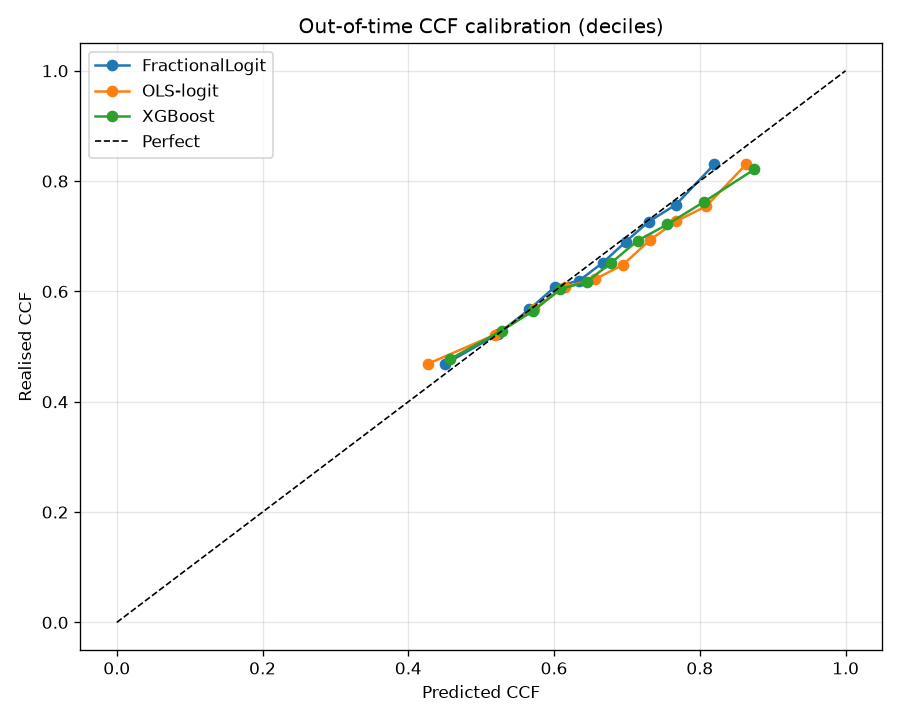
\includegraphics[width=0.85\textwidth]{01_ccf_calibration.png}
\caption{Decile calibration of CCF on the OOT cohort. Fractional logit
tracks the diagonal most closely across the range. All three models
show slight over-prediction at the highest CCF decile because rare
borrowers with $\mathrm{CCF} \to 1$ are hard to distinguish from
$\mathrm{CCF} = 0.8$ borrowers ahead of default.}
\end{figure}

\subsection{Predicted vs realised EAD}

\begin{figure}[H]
\centering
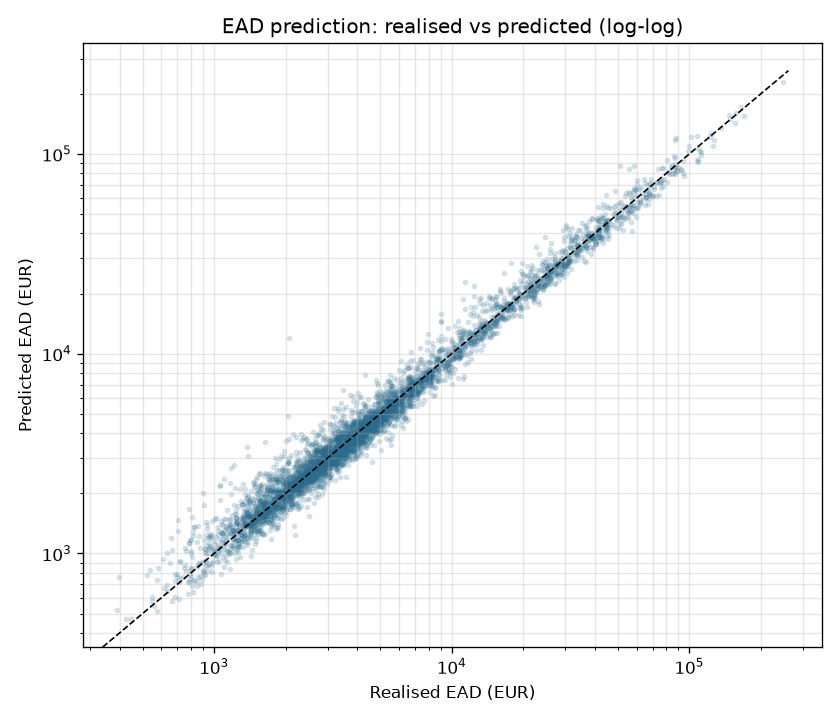
\includegraphics[width=0.7\textwidth]{03_ead_scatter.png}
\caption{Scatter of predicted versus realised EAD on the OOT cohort
(log-log axes). The predictions track the identity line across four
orders of magnitude in EAD.}
\end{figure}

\subsection{CCF by product}

\begin{figure}[H]
\centering
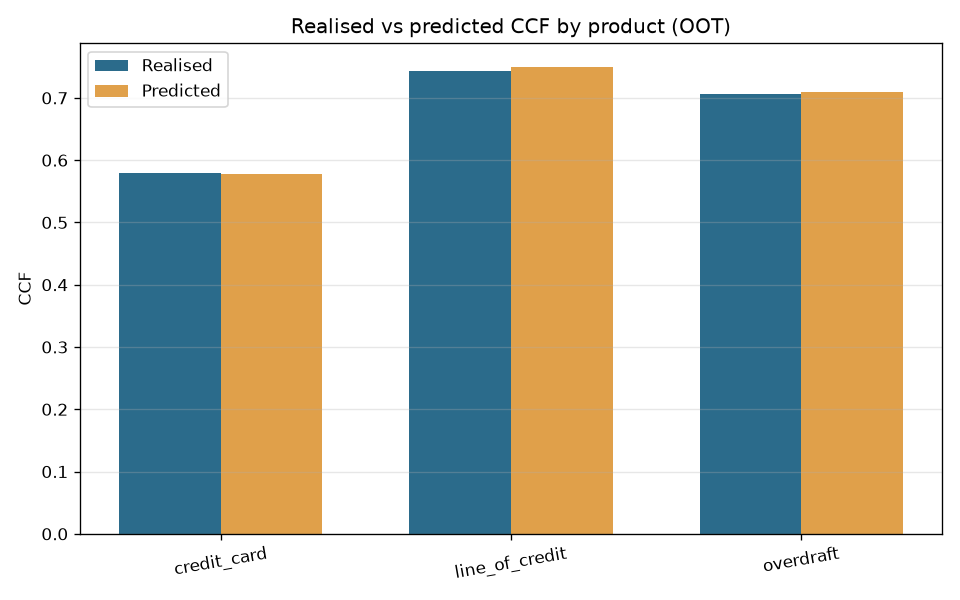
\includegraphics[width=0.75\textwidth]{02_ccf_by_product.png}
\caption{Realised versus predicted mean CCF by product type on the
OOT cohort. Model reproduces the product ordering and the level.}
\end{figure}

\subsection{Downturn CCF}

Basel IRB requires CCF estimates to be downturn-conservative for
regulatory capital. We take the 90th percentile of predicted CCF per
product as the downturn point estimate:

\begin{figure}[H]
\centering
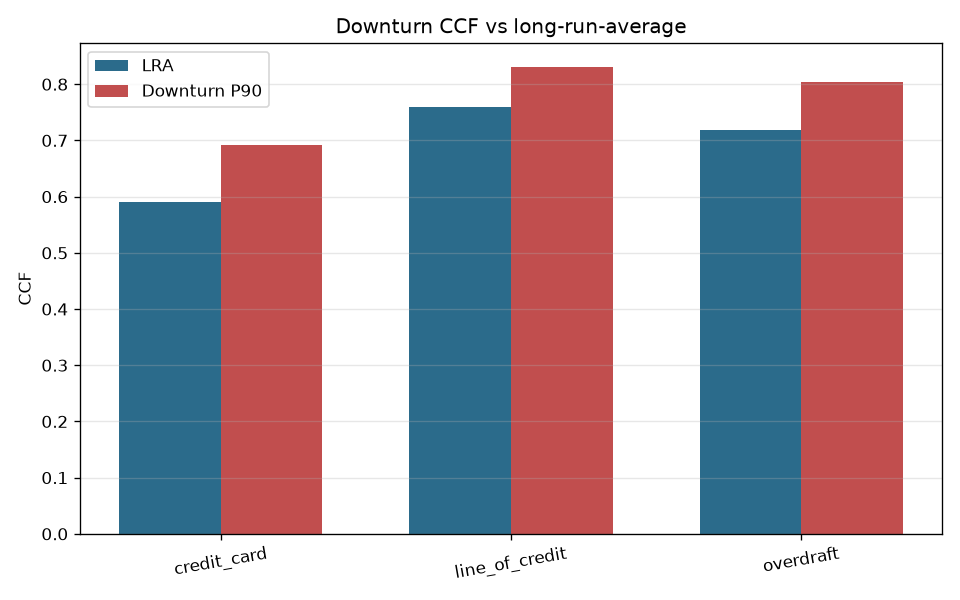
\includegraphics[width=0.75\textwidth]{04_downturn_ccf.png}
\caption{Downturn CCF (P90) versus long-run-average CCF by product.
Credit cards show the largest relative uplift because their LRA is
lowest, leaving more headroom to draw.}
\end{figure}

\subsection{Feature importance}

\begin{figure}[H]
\centering
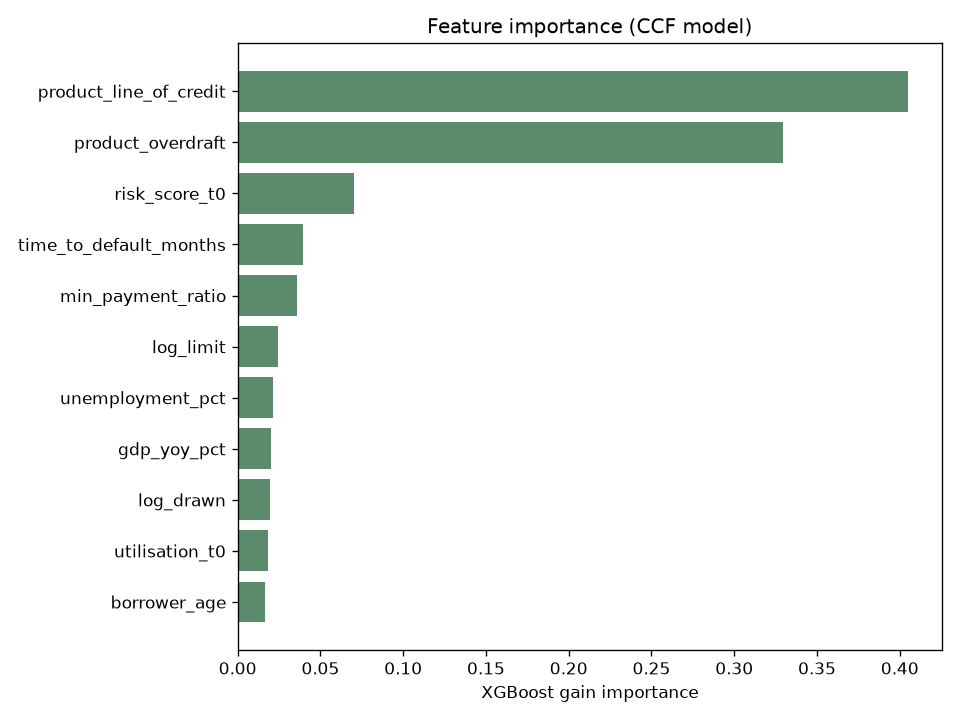
\includegraphics[width=0.8\textwidth]{05_feature_importance.png}
\caption{XGBoost gain importance for the CCF model. Risk score at
$t_0$ is the strongest predictor: high-risk borrowers draw more of
the undrawn commitment before defaulting. Utilisation at $t_0$,
minimum-payment-ratio, and time to default follow.}
\end{figure}

\subsection{Feature stability (PSI)}

Macro-driver PSI is very high between train (2019--2022) and OOT
(2023) because the macro window shifted. Idiosyncratic features
(limit, drawn, risk score, payment ratio, age) are stable.

\begin{table}[H]
\centering
\begin{tabular}{l r}
\toprule
\textbf{Feature} & \textbf{PSI} \\
\midrule
Unemployment pct     & 17.27 \\
GDP YoY              & 16.73 \\
Drawn balance        & 0.010 \\
Credit limit         & 0.003 \\
Min payment ratio    & 0.003 \\
\bottomrule
\end{tabular}
\caption{PSI train vs OOT. As with the LGD model, macro variables
should trigger periodic recalibration; idiosyncratic features are
stable across time.}
\end{table}

\section{Basel IRB and IFRS 9 fit}

\begin{itemize}
  \item \textbf{Basel IRB EAD requirements:} The scorecard produces
        product-level CCF estimates with downturn P90 adjustment. EAD
        for revolving retail is the standard use case for CCF
        modelling under IRB.
  \item \textbf{IFRS 9 lifetime EAD:} Macro-conditional features let
        the CCF respond to forward-looking scenarios, which is
        required for lifetime EAD in stage 2 and 3 exposures.
  \item \textbf{Not fully compliant on:} product-level segmentation
        may be too coarse. Production models typically further split
        by originating channel, tenure, and prior behaviour history.
\end{itemize}

\section{Limitations}

\begin{itemize}
  \item Synthetic panel assumes independent facilities. Real
        portfolios have shared-borrower effects across products.
  \item CCF horizon is fixed at twelve months. Production would use
        multiple horizons (up to a full year of the lifetime for
        IFRS 9).
  \item Utilisation dynamics are simplified. Real drawing behaviour
        follows nonlinear paths near limit that a linear or
        boosted-tree model captures only approximately.
  \item Behavioural features (minimum-payment-ratio) are static at
        $t_0$; in reality they evolve toward default.
\end{itemize}

\section{Files}

\begin{itemize}
  \item \texttt{generate\_data.py} --- synthetic revolving-credit panel
  \item \texttt{train.py} --- CCF pipeline (three models, calibration,
        derived EAD, downturn, PSI)
  \item \texttt{outputs/} --- CCF metrics, EAD metrics, PSI, downturn CSVs
  \item \texttt{figures/} --- five diagnostic plots
\end{itemize}

\end{document}
